\documentclass[11pt]{book}
\usepackage{fontspec}
\setmainfont{TeX Gyre Pagella}
\usepackage[margin=1in]{geometry}
\usepackage{xcolor}
\usepackage{tikz}
\usepackage{amssymb}
\usepackage{enumitem}
\usepackage{titlesec}

\titleformat{\chapter}[display]{\bfseries\Large}{Sproll 00}{0.5em}{\Huge}
\titleformat{\section}{\bfseries\large}{\thesection}{0.6em}{}

\newcounter{algoctr}[section]
\newenvironment{algorithmproc}[1]{%
\vspace{0.6em}\noindent\rule{\linewidth}{0.6pt}\\[0.2em]\textbf{How to Tell: #1}\\[0.3em]}%
{\\[0.2em]\noindent\rule{\linewidth}{0.6pt}\vspace{0.6em}}

\newenvironment{practicenow}{%
\vspace{0.6em}\noindent\rule{\linewidth}{0.6pt}\\[0.2em]\textbf{Practice Now}\\[0.3em]}%
{\\[0.2em]\noindent\rule{\linewidth}{0.6pt}\vspace{0.6em}}

\newenvironment{exercisebox}[1]{%
\vspace{0.8em}\noindent\rule{\linewidth}{0.6pt}\\[0.2em]\textbf{Exercises: #1}\\[0.3em]%
\begin{enumerate}[label=\arabic*., itemsep=0.4em]}%
{\end{enumerate}\noindent\rule{\linewidth}{0.6pt}\vspace{0.6em}}

\newenvironment{trythis}{%
\vspace{0.6em}\noindent\rule{\linewidth}{0.6pt}\\[0.2em]\textbf{Try This}\\[0.3em]}%
{\\[0.2em]\noindent\rule{\linewidth}{0.6pt}\vspace{0.6em}}

\newenvironment{summarybox}{%
\vspace{0.6em}\noindent\rule{\linewidth}{0.6pt}\\[0.2em]\textbf{What We Learned}\\[0.3em]}%
{\\[0.2em]\noindent\rule{\linewidth}{0.6pt}\vspace{0.6em}}

\title{\textbf{Sproll 00}\\[0.3em]\Large A Difference\\[0.5em]\normalsize\textit{a first workbook in the Sproll Curriculum}}
\author{}
\date{}

\begin{document}
\begin{titlepage}
\centering
\vspace*{1.5in}
{\Huge \textbf{SPROLL 00}}\\[0.5in]
{\huge A Difference}\\[0.8in]
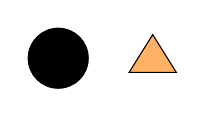
\begin{tikzpicture}
\filldraw[fill=black] (-0.6,0) circle (0.15in);
\draw[fill=orange!60] (0.3,-0.18) -- (0.6,0.3) -- (0.9,-0.18) -- cycle;
\end{tikzpicture}\\[0.8in]
{\Large The Sproll Curriculum}\\[0.2in]
{\large Cycle I: Pops --- Things, Differences, and Counting}
\end{titlepage}

\tableofcontents

\chapter*{Before You Begin}
\addcontentsline{toc}{chapter}{Before You Begin}

Every subject you will ever study in mathematics, from counting to algebra to the strangest ideas in higher math, rests on one small ability: telling one thing apart from everything around it. That sounds almost too simple to be worth a whole workbook. It isn't. Once you start paying close attention to how you tell things apart, you'll notice it is not always as obvious as it looks, and the questions this workbook asks will follow you through every later Sproll in this series.

This book will not ask you to calculate anything. There are no addition problems here, no numbers to find. Its only job is to slow down a skill you already use every day, without ever really thinking about it, so that later books can build on it carefully instead of assuming you already understand it perfectly.

\chapter{What Is a Difference?}

\section{Telling Things Apart}

Look at the two shapes below.

\begin{center}
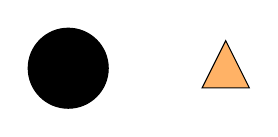
\begin{tikzpicture}
\filldraw[fill=black] (-1,0) circle (0.2in);
\draw[fill=orange!60] (0.7,-0.25) -- (1,0.35) -- (1.3,-0.25) -- cycle;
\end{tikzpicture}
\end{center}

You did not need to be told that these are two different things. A dot is not a triangle. You knew that instantly, without counting anything, without measuring anything, and without anyone explaining a rule to you. That instant judgment, this is one thing, and that is a different thing, is the starting point for this entire workbook, and eventually for a large part of mathematics.

It might seem strange to spend a whole book on something so obvious. Here is why it matters. Before you can count how many things there are, you first have to agree on what counts as one thing. Before you can say two numbers are equal, you first have to know what would make them the same versus merely similar. Before you can group objects into a set, you first have to be able to tell which objects belong together and which do not. Every one of those later skills depends on the ability this workbook is about: recognizing a distinction.

\begin{algorithmproc}{Is This a Difference?}
When you look at two things and want to know whether they are truly different, ask yourself three questions. First, could I point to one of them without also pointing to the other? Second, could I describe one of them in a way that would not also describe the other? Third, if one of them disappeared, would I still notice the other one was there? If the answer to all three is yes, you have found a genuine difference, not just two ways of looking at the same thing.
\end{algorithmproc}

\begin{practicenow}
Look around the room you are in right now. Find two objects that are clearly different from each other. For each one, answer the three questions from the box above out loud or on scrap paper.
\end{practicenow}

\section{Something Does Not Mean Any Particular Kind of Thing}

A common mistake, one this workbook wants to head off early, is to think that being ``a thing'' means being a certain size, or a certain shape, or making a certain amount of noise. It does not. Consider the following four examples, which have almost nothing in common with each other except that each one is, in the sense this book cares about, a single distinguishable something.

A loud clap is something. It lasts only a moment, has no shape you could draw an outline around, and yet you can clearly tell the difference between a room with a clap in it and a room without one.

A quiet, barely audible ring left behind after a bell is struck is also something, even though it is far fainter than the clap, harder to notice, and fades away rather than stopping all at once.

A shadow cast on the ground by an object out of view is something too, even though a shadow, unlike the dot or the triangle from before, is not really a solid object at all. It is an absence of light with a definite edge.

A large, messy scribble with no recognizable shape is also something, even though it does not look like any object you could name. It is still one distinguishable mark, different from the blank page around it.

\begin{trythis}
For each of the four examples above, the clap, the ring, the shadow, and the scribble, write down one thing they have in common (besides all being examples in this book) and one way they are different from each other.
\end{trythis}

\begin{summarybox}
Something does not mean big, and it does not mean loud, and it does not mean round. Something just means: here it is, distinguishable from what surrounds it, however briefly or faintly.
\end{summarybox}

\begin{exercisebox}{Section 1.2}
\item List three things in your own life, from today or yesterday, that count as ``something'' in the sense of this workbook, but that are not solid objects you could pick up. (Hint: think about sounds, smells, feelings of temperature, or moments in time.)
\item Explain in one or two sentences why a shadow counts as a distinguishable something even though it is not made of any material.
\item A song on the radio ends and the room goes quiet. Is the silence afterward ``something,'' in the sense this workbook is using the word? Explain your reasoning either way.
\end{exercisebox}

\chapter{Alike, But Are They the Same?}

\section{Two Marks That Look Identical}

Now consider a harder case. Below are two dots, drawn to look exactly alike: same size, same color, same shape.

\begin{center}

\begin{tikzpicture}
\filldraw[fill=black] (-1.5,0) circle (0.16in);
\filldraw[fill=black] (1.5,0) circle (0.16in);
\end{tikzpicture}
\end{center}

They look alike. But are they the same thing, or are they two different things that merely resemble each other closely? This is not a trick question, and this workbook is not going to give you a final answer to it here. It is worth sitting with the question honestly rather than rushing to settle it.

Here is one way to think about it. The two dots occupy different places on the page. One is on the left, the other on the right. If you could only see one of them at a time, moved so that its position matched the other's exactly, you might not be able to tell which one you were looking at. But right now, side by side, you can clearly point to ``the left one'' and ``the right one'' separately. That already tells you something important: looking alike and being identical are not automatically the same thing.

Think about two brand-new pennies fresh from a coin factory, stamped from the same machine on the same day. They can look completely identical, down to the smallest detail visible to the eye. And yet you would still say there are two pennies, not one penny counted twice. What makes them two, if not any visible difference?

\begin{algorithmproc}{Alike Versus Same}
Two things looking alike tells you about their appearance. Two things being the same, or not, is a separate question, about their identity. A useful habit is to ask: if I swapped these two things with each other right now, would anything in the world actually change? If the honest answer is no, that is evidence, though not final proof, that appearance is doing all the work here, and identity is a separate matter still worth thinking about.
\end{algorithmproc}

\begin{exercisebox}{Section 2.1}
\item Name two objects in your daily life that look almost exactly alike (for example, two socks from the same pair, two identical pencils, two leaves from the same tree) and explain what, if anything, makes them different objects rather than one object seen twice.
\item Twins can look extremely similar. Explain, in your own words, why looking similar does not mean two people are ``the same person.''
\item Can you think of a case where two things that look completely different are, in some important sense, the same thing? (Hint: think about a caterpillar and the butterfly it becomes, or a glass of water and the ice cube it was frozen from.)
\end{exercisebox}

This last exercise question is worth pausing on, because it points in the opposite direction from the dots. Sometimes two things that look nothing alike turn out to be connected in an important way, and sometimes two things that look exactly alike turn out to be genuinely separate. This workbook is not going to resolve that tension yet. A much later Sproll in this series, once you have more tools available, returns to exactly this question and gives it a precise answer. For now, the important habit is simply noticing that ``looks the same'' and ``is the same'' are two different claims, which do not always agree.

\chapter{Can Many Things Be Treated as One?}

\section{A Group Inside a Boundary}

Picture a small cluster of objects: a couple of dots, a triangle, and a squiggly mark, all sitting close together, with a circle drawn around the whole group to mark it off from the rest of the page.

\begin{center}
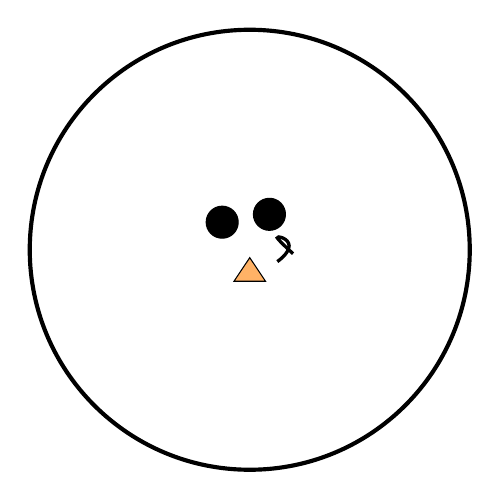
\begin{tikzpicture}
\draw[line width=1.5pt] (0,0) circle (1.1in);
\filldraw[fill=black] (-0.35,0.35) circle (0.08in);
\filldraw[fill=black] (0.25,0.45) circle (0.08in);
\draw[fill=orange!60] (-0.2,-0.4) -- (0,-0.1) -- (0.2,-0.4) -- cycle;
\draw[line width=1.2pt] plot [smooth, tension=1.2] coordinates
{(0.35,-0.15) (0.5,0.05) (0.35,0.15) (0.55,-0.05)};
\end{tikzpicture}
\end{center}

Here is a genuine puzzle. Is what's inside the boundary one thing, because it is a single group with a boundary drawn around it, or is it four things, because there are clearly four separate marks inside? The honest answer is: sometimes one, sometimes four, depending entirely on what question you are asking and what you plan to do next.

Think about a stack of one hundred pennies. If you are asked ``how much money is this,'' you treat the stack as one amount, one dollar. If you are asked ``how many coins are in this stack,'' the very same stack is suddenly one hundred separate things. Nothing about the pennies changed between those two questions. What changed was the rule you were using to look at them.

A sports team works the same way. A team can win a game, lose a game, or have a certain record for the season, and in each of those sentences the team is being treated as one thing. But that same team also has eleven, or nine, or five separate players, each with a name, a position, and statistics of their own, and in that context the team is obviously many things, not one. Both descriptions are correct. They are just correct under different rules for what counts as ``one.''

\begin{trythis}
Think of one more everyday example, besides pennies and sports teams, where the same collection of objects can honestly be counted as ``one thing'' under one rule and as ``many things'' under a different rule. Write down both rules explicitly.
\end{trythis}

\begin{summarybox}
Many things can be treated as one, but only relative to a rule for what counts as ``one'' in that situation. The same objects, looked at under a different rule, might just as honestly be counted as many. Neither rule is the real, final answer; each rule answers a different question. A later Sproll in this series names this idea precisely and gives you the tools to state exactly which rule is being used in any given case.
\end{summarybox}

\begin{exercisebox}{Section 3.1}
\item A library shelf holds twenty books. Under what rule is the shelf ``one thing''? Under what rule is it ``twenty things''? Write both rules in your own words.
\item A single sentence is made of several words, and each word is made of several letters. Explain how the same piece of writing can honestly be described as one sentence, several words, or many letters, depending on the rule being used.
\item Challenge: can you think of a case where it is genuinely unclear which rule should apply, so that reasonable people might disagree about whether something counts as one thing or many? Describe it.
\end{exercisebox}

\chapter*{Looking Ahead}
\addcontentsline{toc}{chapter}{Looking Ahead}

This workbook has deliberately left two questions open rather than answering them. Are two things that look exactly alike really the same, or really different? And when is a group of things correctly counted as one, and when as many? Both questions will return later in the Sproll Curriculum, once you have new tools, in particular a way of stating exactly what rule you are using to look at something. For now, the goal was only to notice that these are real questions, worth asking carefully, rather than obvious ones with an answer everyone already agrees on.

The next workbook in this series, Sproll 01: Something Happened, begins from a different kind of question: not what can be distinguished, but what happens when you actually choose one thing out of several possible things. That turns out to require a new idea entirely, one this workbook has not yet introduced.

\chapter*{For Parents and Teachers}
\addcontentsline{toc}{chapter}{For Parents and Teachers}

This workbook is the first in a forty-book mathematics curriculum built on a formal system of historical construction, in which mathematical objects and facts are treated as arising from a sequence of committed actions rather than as static, pre-existing truths. Nothing in that underlying formalism is stated explicitly in this book; it is deliberately withheld until Sproll 01 and later booklets have given the child concrete experience to attach it to.

This book's specific job is to establish individuation, the ability to tell one thing apart from its surroundings, as a genuine prerequisite skill rather than something to be assumed. Two questions are raised and deliberately left unresolved: whether two indistinguishable-looking things are really the same, and whether a group of things is correctly counted as one or as many. Both are real, substantive questions in the mathematics this curriculum eventually develops, not simplifications invented for a young reader, and both receive precise treatment later in the series once the necessary vocabulary exists. Resolving them here would either be dishonest about how difficult the questions actually are, or would require introducing machinery this book is not yet ready to support.

If your child wants a definite answer to either open question, it is entirely appropriate to say that mathematicians themselves need careful tools to answer these questions precisely, and that this curriculum will build exactly those tools over its next several books.

\end{document}
